% Apéndices: elaboración propia. Se numeran A, B, ... (\apendice en tesis-usach.tex)

\chapter{Fichas de los avances}
\label{ap:avances}

Cada avance se describe con el formato de \citet{figueroa2025arquitectura}: identificador, nombre, objetivos, descripción y requisitos funcionales y no funcionales. Las tablas se generan desde la carpeta \texttt{avances/} del repositorio.

{\small% Tablas de prototipos de EDDIE (formato de Figueroa Contreras, 2025). Requiere \usepackage{tabularx}.
% Generado desde avances/; revisa los códigos de requisitos antes de usarlos.

% ---------------- P-01
\begin{table}[h!]
\centering
\caption{Primer prototipo - Núcleo orquestador y contratos de plugins.}
\label{tab:prototipo-p01}
\begin{tabularx}{\textwidth}{|l|X|}
\hline
ID Prototipo & P-01 \\ \hline
Nombre & Núcleo orquestador y contratos de plugins \\ \hline
Objetivos & Definir PluginBase y los contratos de cada módulo (ICameraSensor, IImageProcessor, IGesturePlugin, IEyeTracker, IConsistencyProvider, IWebSearchProvider, ISpeechProvider). \newline Implementar el OrchestratorCore (inicializar $\rightarrow$ ejecutar $\rightarrow$ liberar) y el PluginLoader con un único mecanismo de carga. \newline Validar la inyección de dependencias sensor$\rightarrow$consumidor, el aislamiento de fallos y la latencia por ciclo. \\ \hline
Descripción & Primera versión del núcleo, sin interfaz. Se prueba con dispositivos simulados (MockCameraSensor, EyeTrackerMock) y con plugins de prueba: un consumidor de frames, un consumidor de resultados del ciclo, un plugin que falla cada 10 ciclos y una entrada con una clase inexistente (equivalente a la DLL faltante de los errores E38/E50). El OrchestratorCore de este avance es la versión temprana del repositorio (sin overrides, invoke ni reinicio en caliente). \\ \hline
Requisitos Funcionales & N1, N2, N3, RFCO12 \\ \hline
Requisitos No Funcionales & RNF-01, RNF-02, RNF-04, RNF-05 \\ \hline
\end{tabularx}
\\[2pt] {\small Fuente: Elaboración propia, 2026.}
\end{table}

% ---------------- P-02
\begin{table}[h!]
\centering
\caption{Segundo prototipo - Capa de abstracción de hardware y módulo de consistencia.}
\label{tab:prototipo-p02}
\begin{tabularx}{\textwidth}{|l|X|}
\hline
ID Prototipo & P-02 \\ \hline
Nombre & Capa de abstracción de hardware y módulo de consistencia \\ \hline
Objetivos & Incorporar DeviceFactory para conmutar cada dispositivo entre real y simulado sin cambiar código. \newline Implementar la cámara real (OpenCV, hilo de captura) y la enumeración de cámaras de Windows. \newline Integrar primero el módulo sin dependencia de hardware: la consistencia papel$\leftrightarrow$PDF como plugin IConsistencyProvider (PyMuPDF). \newline Extender el núcleo con overrides de configuración, invocación bajo demanda, reinicio en caliente y traza de ejecución. \\ \hline
Descripción & El núcleo pasa a su versión definitiva y se agrega la capa HAL. La consistencia (resaltados, marcadores, comentarios y figuras, búsqueda de texto) se ejecuta a través del orquestador con OrchestratorCore.invoke(). Sigue sin interfaz: se demuestra con demos/demo\_consistencia.py, que sincroniza tres <<fotos>> sintéticas de la hoja con un PDF de prueba y guarda el PDF resultante y el render de cada página. \\ \hline
Requisitos Funcionales & N4, N5, N6, N8, C1, C2, C3, C7, C9, C10, C11 (parcial) \\ \hline
Requisitos No Funcionales & RNF-01, RNF-02, RNF-04, RNF-05 \\ \hline
\end{tabularx}
\\[2pt] {\small Fuente: Elaboración propia, 2026.}
\end{table}

% ---------------- P-03
\begin{table}[h!]
\centering
\caption{Tercer prototipo - Reconocimiento de texto e interfaz de configuración.}
\label{tab:prototipo-p03}
\begin{tabularx}{\textwidth}{|l|X|}
\hline
ID Prototipo & P-03 \\ \hline
Nombre & Reconocimiento de texto e interfaz de configuración \\ \hline
Objetivos & Integrar el reconocimiento del texto resaltado (IImageProcessor: segmentación del resaltado + Tesseract) sobre la cámara de texto declarada. \newline Construir la ventana de configuración a partir de los controles extraídos de los .Designer.cs, con un diseño propio en español (ui/theme.py, ui/modern\_forms.py) y las páginas Texto (OCR) y Documento PDF. \newline Ejecutar el ciclo del orquestador dentro de Qt (EddieRuntime) y persistir los ajustes. \newline Poder probar el OCR y ver el PDF cargado desde estas páginas, sin esperar la pantalla de proyección. \\ \hline
Descripción & Aparece la interfaz. Conserva todos los controles del original (mismo nombre, tipo, rangos y estado inicial), ordenados en tarjetas con layouts de Qt, con un menú lateral que muestra el estado de cada módulo y una pantalla de inicio <<Preparar sesión>>. Solo se construyen las páginas de los módulos ya integrados: las demás aparecen en el menú deshabilitadas con el avance en que se integran, y <<Iniciar proyección>> avisa que la proyección llega en P-06. Como en el C\# el texto reconocido solo se veía desde la proyección, se agregan el botón <<Reconocer texto>> con el texto reconocido y una vista previa del PDF con navegación de páginas. Los mensajes son avisos no modales. \\ \hline
Requisitos Funcionales & FD1, N7, U1, U3, RFS3, RFS5, RFS6, RFS7, RFS8 \\ \hline
Requisitos No Funcionales & RNF-01, RNF-06, RNF-07 \\ \hline
\end{tabularx}
\\[2pt] {\small Fuente: Elaboración propia, 2026.}
\end{table}

% ---------------- P-04
\begin{table}[h!]
\centering
\caption{Cuarto prototipo - Interacción gestual.}
\label{tab:prototipo-p04}
\begin{tabularx}{\textwidth}{|l|X|}
\hline
ID Prototipo & P-04 \\ \hline
Nombre & Interacción gestual \\ \hline
Objetivos & Integrar los plugins gestuales del C\# (Color Pen, Hand Skin, Mouse) bajo IGesturePlugin, compartiendo la cámara gestual declarada. \newline Portar la calibración sensor$\rightarrow$aplicación, el control del cursor (<<Recognition on>>), la máquina de estados del clic y la captura automática de la selección. \newline Agregar la página Gestos, con calibración asistida (<<Fijar inicio>> / <<Fijar fin>> desde la lectura del sensor). \\ \hline
Descripción & Los tres detectores heredan una base común (CalibratedGesturePlugin) que aplica la calibración y el clic; cada uno solo implementa su detección. Este avance porta el comportamiento del C\# tal cual, incluida la rotación fija de 180$^{\circ}$ de Hand Skin, que después se detectó como defecto (H-01). \\ \hline
Requisitos Funcionales & G1, G2, G3, U2 \\ \hline
Requisitos No Funcionales & RNF-01, RNF-04, RNF-06 \\ \hline
\end{tabularx}
\\[2pt] {\small Fuente: Elaboración propia, 2026.}
\end{table}

% ---------------- P-05
\begin{table}[h!]
\centering
\caption{Quinto prototipo - Rastreo ocular.}
\label{tab:prototipo-p05}
\begin{tabularx}{\textwidth}{|l|X|}
\hline
ID Prototipo & P-05 \\ \hline
Nombre & Rastreo ocular \\ \hline
Objetivos & Unificar GazePoint (Open Gaze API), TheEyeTribe y GazeCloud bajo IEyeTracker, con EyeTrackerMock como contingencia (DeviceFactory). \newline Portar la sesión de mirada: control del mouse por mirada, clic por permanencia, retícula y registro CSV. \newline Agregar la página Rastreo ocular (exportar/importar configuración). \\ \hline
Descripción & Los tres protocolos se prueban con servidores falsos que emiten el mismo formato que los dispositivos reales. La sesión de mirada es un consumidor de resultados del ciclo: recibe la muestra del eye tracker en el mismo ciclo en que se produce. \\ \hline
Requisitos Funcionales & RO1–RO7, RFS4 \\ \hline
Requisitos No Funcionales & RNF-01, RNF-02, RNF-05 \\ \hline
\end{tabularx}
\\[2pt] {\small Fuente: Elaboración propia, 2026.}
\end{table}

% ---------------- P-06
\begin{table}[h!]
\centering
\caption{Sexto prototipo - Pantalla de proyección, búsqueda con LLM y voz.}
\label{tab:prototipo-p06}
\begin{tabularx}{\textwidth}{|l|X|}
\hline
ID Prototipo & P-06 \\ \hline
Nombre & Pantalla de proyección, búsqueda con LLM y voz \\ \hline
Objetivos & Integrar la pantalla de proyección (ProjectionScreenActivity2): modo resaltado/captura, búsqueda y sincronización papel$\leftrightarrow$PDF, con los botones en la franja superior (zona de mayor validez del eye tracker según Ibaceta, 2023) y la zona de lectura y las cruces en su posición original. \newline Responder los cinco servicios de búsqueda con Gemini 2.5 Flash bajo IWebSearchProvider, en lugar de las APIs vencidas (Wikipedia, Google, Bing, YouTube, Cloud Vision). \newline Integrar lectura en voz alta y comandos de voz (ISpeechProvider) y las páginas Interacción y Búsquedas. \\ \hline
Descripción & Con este avance el sistema queda completo y equivale al código de <<Proyecto final>> antes de la verificación. Es una extensión respecto del alcance del seminario, donde IWebSearchProvider quedaba solo como interfaz. \\ \hline
Requisitos Funcionales & B1–B13, C5, C6, C8, C11, C12, RFS1, RFS2 \\ \hline
Requisitos No Funcionales & RNF-01, RNF-06, RNF-08 \\ \hline
\end{tabularx}
\\[2pt] {\small Fuente: Elaboración propia, 2026.}
\end{table}

% ---------------- P-07
\begin{table}[h!]
\centering
\caption{Séptimo prototipo - Versión final verificada.}
\label{tab:prototipo-p07}
\begin{tabularx}{\textwidth}{|l|X|}
\hline
ID Prototipo & P-07 \\ \hline
Nombre & Versión final verificada \\ \hline
Objetivos & Verificar el sistema integrado: cobertura, latencia, trazabilidad de errores y pruebas de regresión. \newline Corregir los hallazgos de la verificación (H-01, H-02, H-03) y dejar una prueba que los detecte. \newline Cerrar la documentación técnica (README, EQUIVALENCIAS, DISENO\_INTERFAZ). \\ \hline
Descripción & Es el contenido de <<Proyecto final>> con las correcciones de la verificación. Cada hallazgo tiene una prueba de regresión que falla con el código de P-06 y pasa con el de P-07. \\ \hline
Requisitos Funcionales & Todos los anteriores \\ \hline
Requisitos No Funcionales & RNF-01, RNF-02, RNF-03, RNF-04, RNF-05, RNF-06, RNF-07, RNF-08 \\ \hline
\end{tabularx}
\\[2pt] {\small Fuente: Elaboración propia, 2026.}
\end{table}

% ---------------- Hallazgos (fase de reparación MECIVA PS)
\begin{table}[h!]
\centering
\caption{Hallazgos de la verificación.}
\label{tab:hallazgos}
\begin{tabularx}{\textwidth}{|l|X|l|X|}
\hline
ID & Descripción & Estado & Justificación o Solución \\ \hline
H-01 & Al calibrar con Hand Skin la vista de la cámara aparece rotada 180$^{\circ}$. HandSkinRecognition.cs rotaba siempre la imagen porque la cámara del laboratorio estaba montada invertida; el port conservó esa rotación fija, solo en ese plug-in (Color Pen y Mouse no rotan), así que la vista previa y las coordenadas de calibración quedaban al revés con cualquier otra cámara. & SF & La rotación pasa a ser una opción común de los tres plug-ins (rotate\_180, por defecto desactivada) que se aplica una sola vez al frame; vista previa, coordenadas y recorte comparten orientación. Casilla nueva <<Rotar la imagen 180$^{\circ}$>> en Gestos para el montaje invertido del laboratorio. \\ \hline
H-02 & ConsistencyPlugin guardaba cada cambio con saveIncr(). Con PyMuPDF 2.1, desde el segundo guardado incremental el PDF queda con la xref dañada; al reabrirlo PyMuPDF lo <<repara>> y se pierden los resaltados, comentarios y marcadores guardados antes. En pantalla no se notaba porque el documento en memoria seguía correcto. & SF & Cada guardado escribe una copia completa en un archivo temporal, reemplaza el original y vuelve a abrirlo (se mantiene el respaldo .bac). Si otro programa tiene el PDF bloqueado (Windows), se reintenta y luego se informa con un mensaje claro. \\ \hline
H-03 & Al pulsar los botones de carpeta o las casillas de Rastreo ocular aparecía <<'bool' object has no attribute 'mapToGlobal'>>. La ayuda contextual se conectaba con lambda w=widget, t=text a la señal clicked; en los botones, clicked(bool) entrega checked y Qt lo pasaba como primer argumento, reemplazando w por False. La acción del botón sí se ejecutaba, pero cada clic dejaba una excepción. & SF & La ayuda por clic queda solo para los íconos de información; los botones y casillas la muestran al pasar el mouse. La lambda ignora los argumentos de la señal (lambda *\_, w=widget, t=text). Se corrige desde P-05, primer avance con esos controles, hasta P-07. \\ \hline
\end{tabularx}
\\[2pt] {\small Fuente: Elaboración propia, 2026.}
\end{table}
}

\chapter{Mediciones de los prototipos}
\label{ap:mediciones}

La Tabla~\ref{tab:resumen_mediciones} resume el tipo de medición y el resultado principal de cada prototipo. El detalle (protocolo, fórmula, parámetros y todas las métricas) está en \texttt{avances/P-00\_prototipos\_desechables/evidencias/MEDICIONES.md}, generado junto con los valores de este documento.

\begin{table}[H]
\centering
\caption{Resumen de las mediciones de los prototipos.}
\label{tab:resumen_mediciones}
\footnotesize
\begin{tabularx}{\textwidth}{l l >{\raggedright\arraybackslash}X}
\toprule
\textbf{ID} & \textbf{Tipo} & \textbf{Resultado principal} \\ \midrule
F1 & \FUnoTipo & \pendiente{FPS y latencia con las cámaras} \\
F2 & \FDosTipo & Eficacia Otsu \FDosEficaciaPct\%; adaptativo \FDosEficaciaAdaptativoPct\% \\
F3 & \FTresTipo & CER \FTresCerLimpioPct\% / WER \FTresWerLimpioPct\% (sin preproceso: \FTresCerSinPreprocesoPct\% / \FTresWerSinPreprocesoPct\%) \\
F4 & \FCuatroTipo & Éxito \FCuatroExitoPct\%, RMSE \FCuatroRmsePx~px \\
F5 & \FCincoTipo & Detección \FCincoDeteccionPct\% sin rojo proyectado; \FCincoDeteccionRojoPct\% con rojo \\
F6 & \FSeisTipo & IoU \FSeisIouPct\%, punta correcta \FSeisPuntaOkPct\% \\
F7 & \FSieteTipo & Error de reproyección \FSieteErrorPx~$\pm$~\FSieteErrorSdPx~px \\
F9 & \FNueveTipo & \pendiente{latencia de eventos} \\
F10 & \FDiezTipo & Pérdida \FDiezPerdidaPct\%, \textit{jitter} \FDiezJitterMs~ms \\
F11 & \FOnceTipo & \FOnceFallas{} fallas en \FOnceCargas{} cargas, \FOnceTiempoMs~ms \\
F12 & \FDoceTipo & \FDoceVoluntariasPct\% voluntarias, \FDoceAccidentalesPorMin{} accidentales/min \\
F13 & \FTreceTipo & \FTreceTiempoMs~ms por cuadro \\
F14 & \FCatorceTipo & Coherencia \FCatorceCoherenciaPct\% \\
F15 & \FQuinceTipo & \FQuincePersistidas{}/\FQuinceAnotaciones{} persistidos, \FQuinceTiempoMs~ms \\
F16 & \FDieciseisTipo & \FDieciseisDetectadasPct\% detectadas, \FDieciseisErrorPt~pt \\
F17 & \FDiecisieteTipo & Exactitud \FDiecisieteExactitudPct\%, IoU \FDiecisieteIouPct\% \\
F24 & \FVeinticuatroTipo & \pendiente{exactitud de comandos} \\
F25 & \FVeinticincoTipo & \pendiente{palabras por minuto} \\
F27 & \FVeintisieteTipo & \FVeintisieteTiempoMs~ms por cuadro \\ \bottomrule
\end{tabularx}
\fuente{Elaboración propia, \texttt{mediciones/medir\_prototipos.py} (P-00), \MedicionFecha.}
\end{table}

Para repetir las mediciones en el PC y agregar las de hardware:
\begin{verbatim}
cd avances\P-00_prototipos_desechables
python mediciones\medir_prototipos.py --pdf ruta\al\documento.pdf --camara 0
python ..\..\tesis\datos\actualizar_datos.py ..
\end{verbatim}
El segundo comando copia los valores nuevos a \texttt{datos/}, y al recompilar el documento todas las tablas y fichas se actualizan.

\chapter{Comparación de la interfaz}
\label{ap:interfaz}

Las figuras siguientes comparan la interfaz de EDDIE-2023, reproducida a partir de sus archivos \texttt{.Designer.cs}, con la versión en Python.

\begin{figure}[H]
\centering
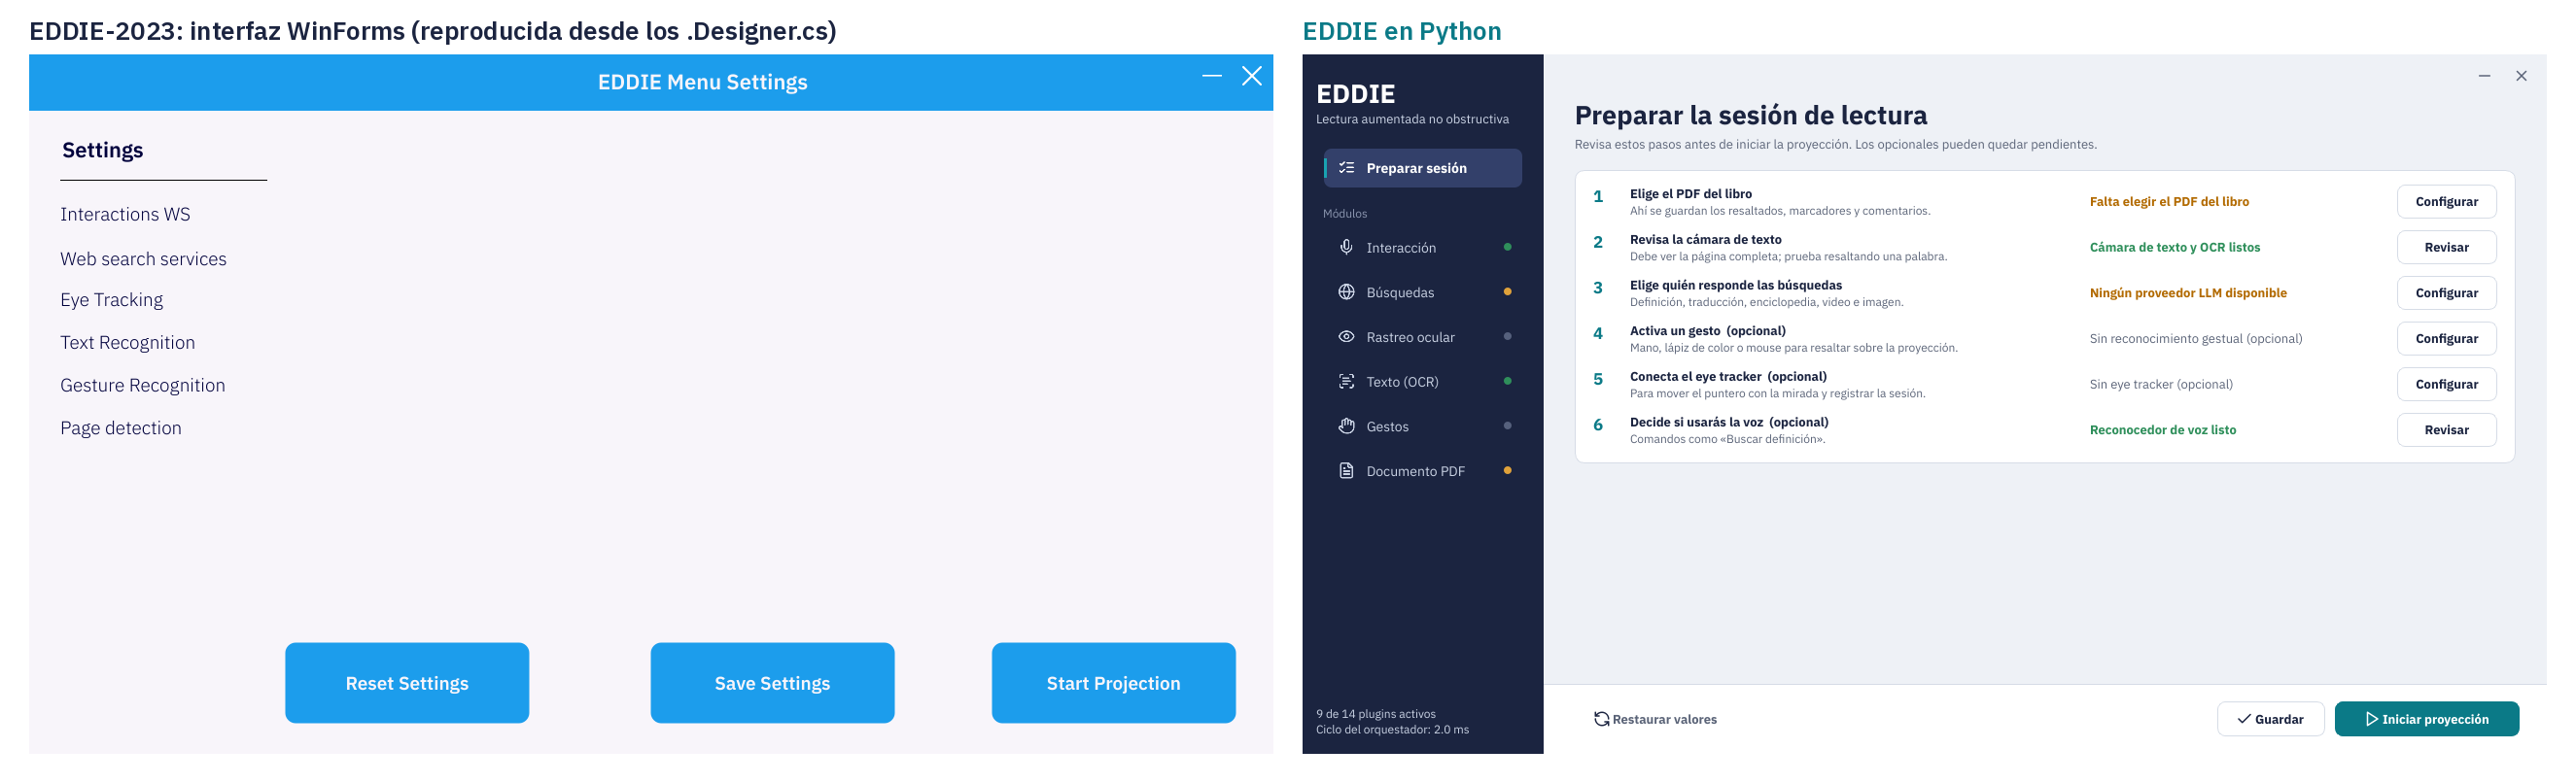
\includegraphics[width=\textwidth]{figuras/comparacion_inicio.png}
\caption{Pantalla de inicio: EDDIE-2023 (izquierda) y versión en Python (derecha).}
\fuente{Elaboración propia.}
\end{figure}

\begin{figure}[H]
\centering
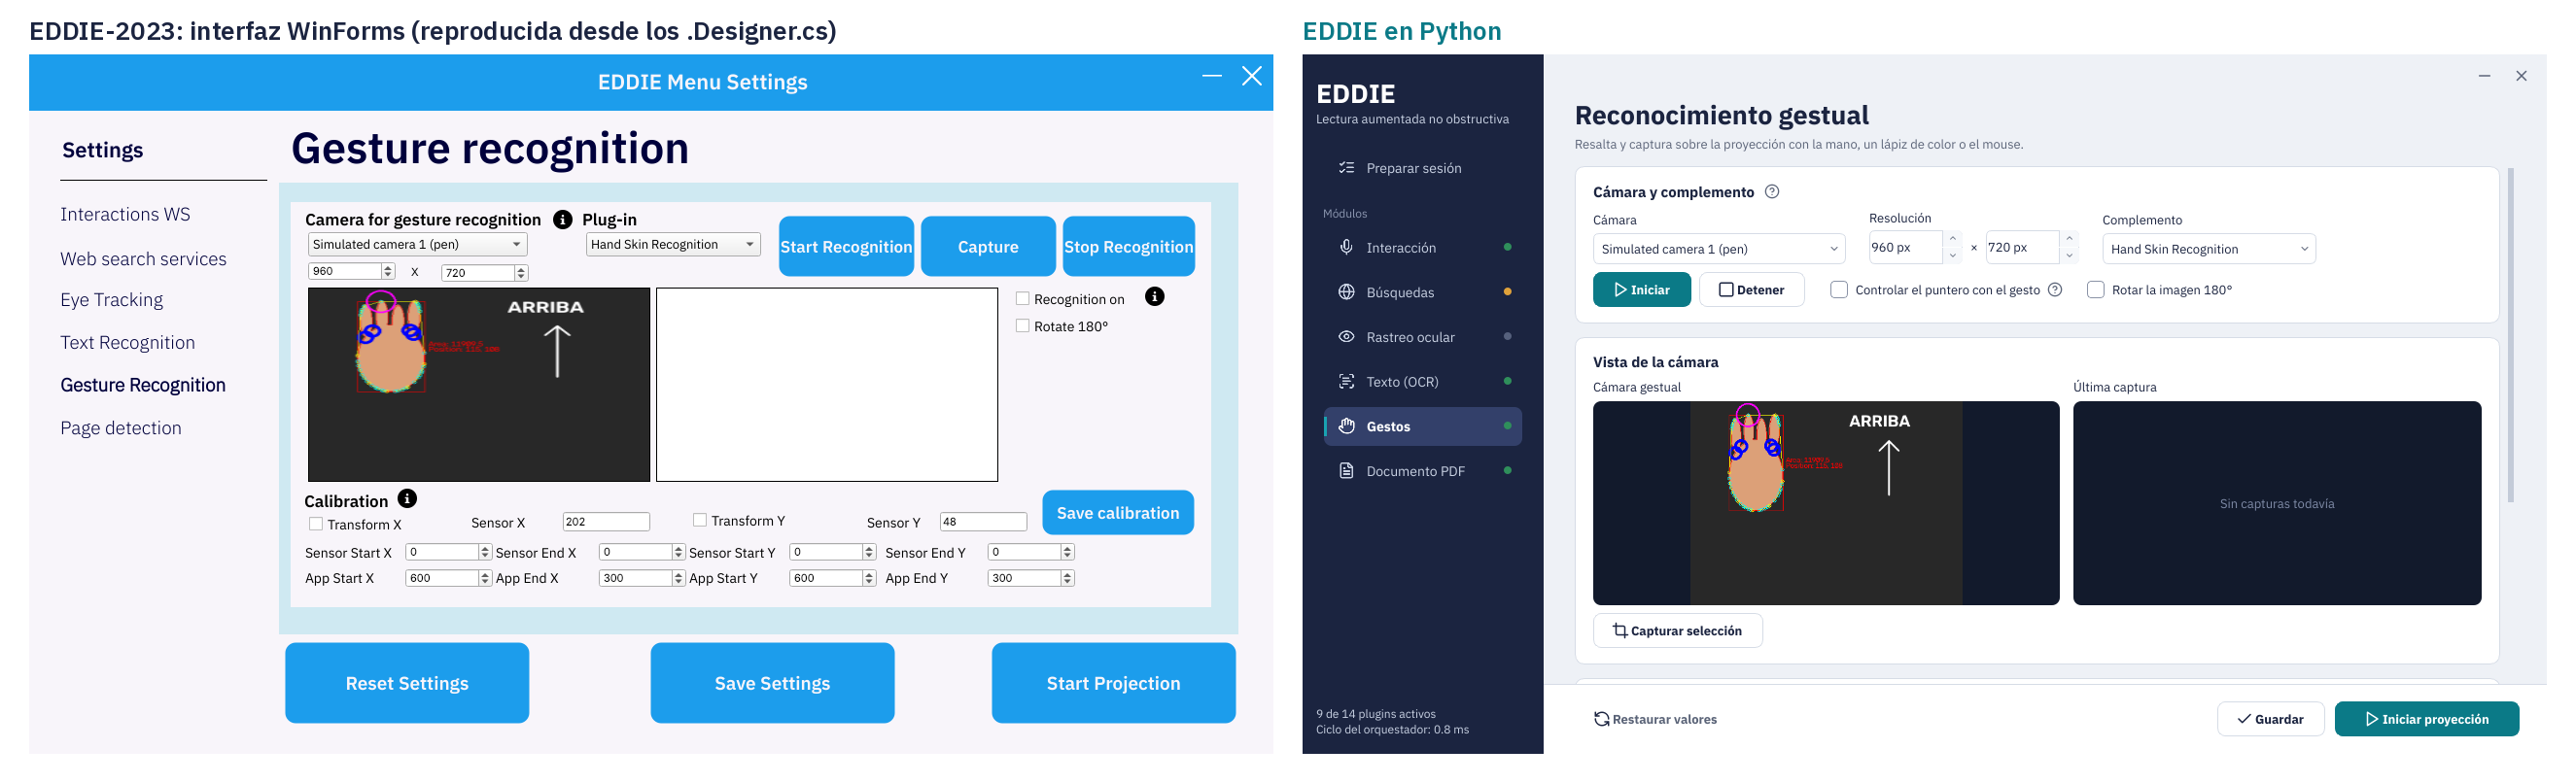
\includegraphics[width=\textwidth]{figuras/comparacion_gestos.png}
\caption{Configuración de gestos: EDDIE-2023 (izquierda) y versión en Python (derecha).}
\fuente{Elaboración propia.}
\end{figure}

\begin{figure}[H]
\centering
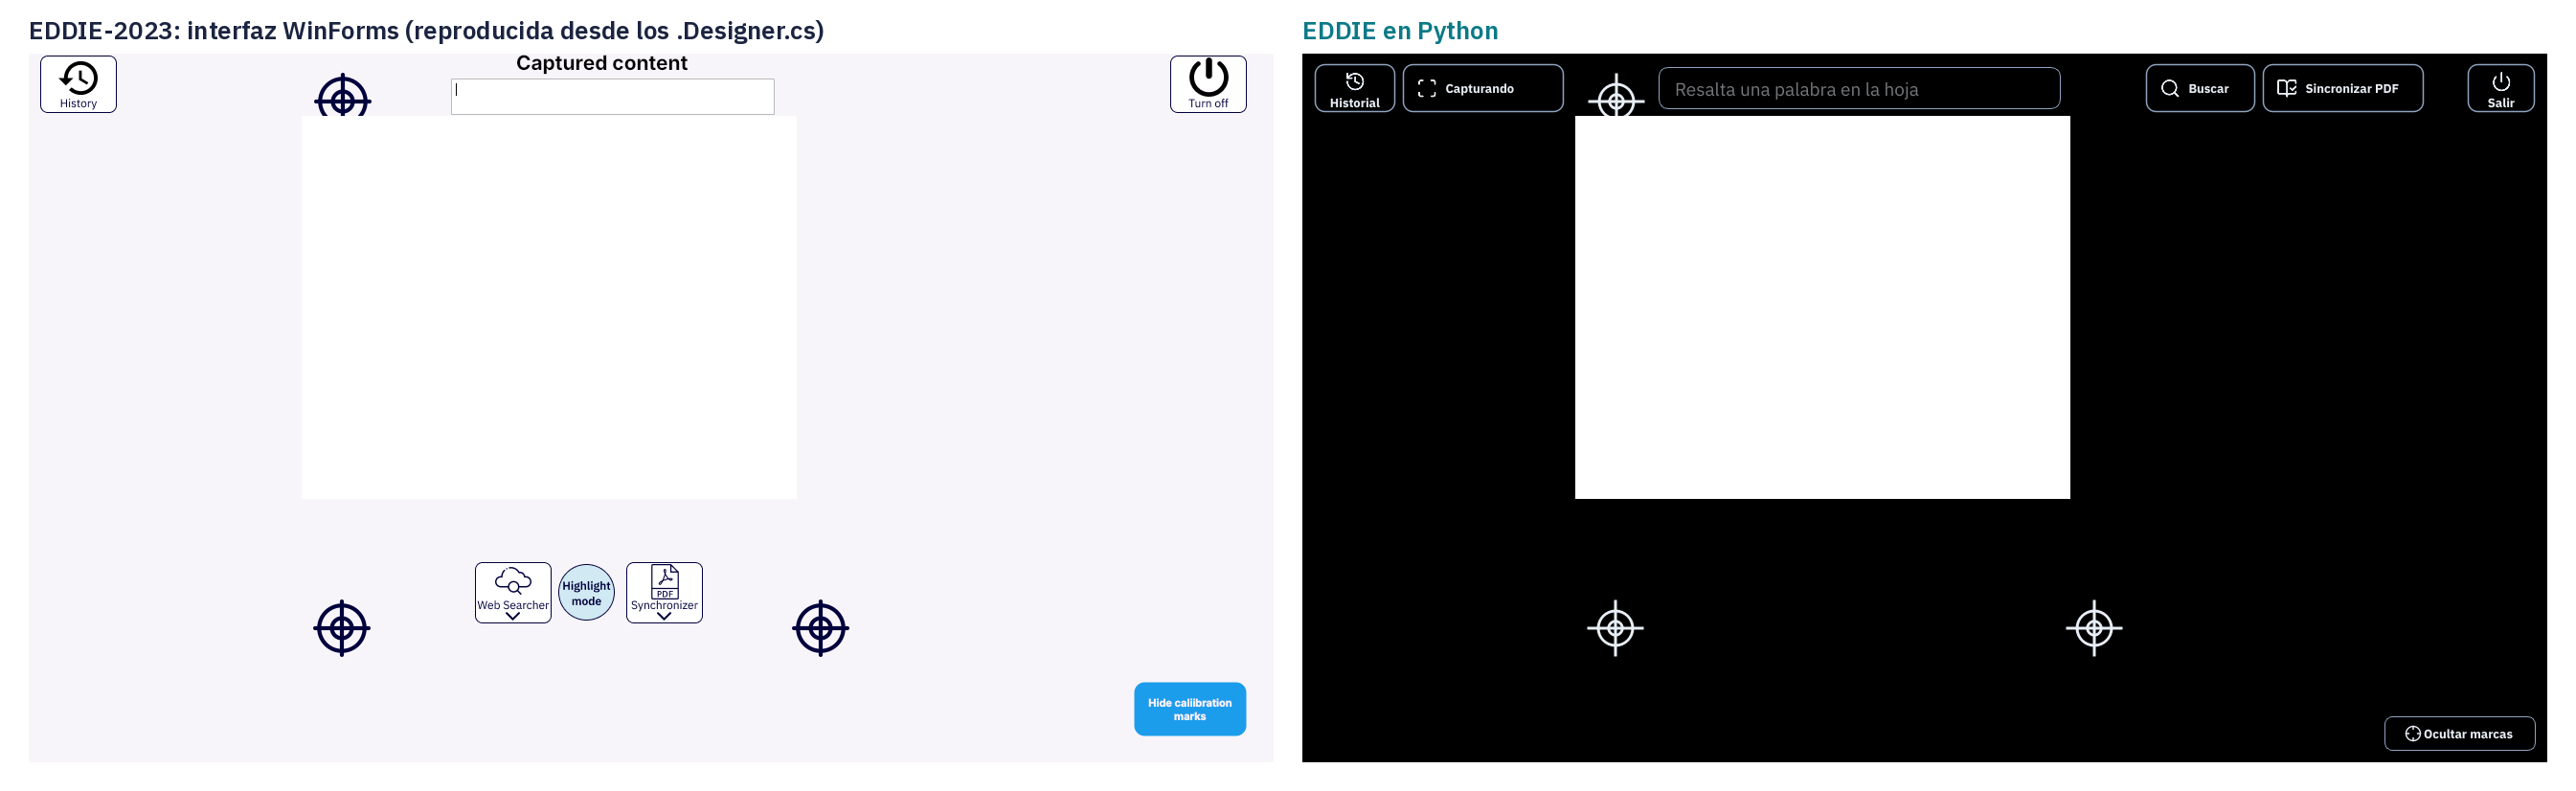
\includegraphics[width=\textwidth]{figuras/comparacion_proyeccion.png}
\caption{Pantalla proyectada: EDDIE-2023 (izquierda) y versión en Python (derecha).}
\fuente{Elaboración propia.}
\end{figure}

\chapter{Manual de instalación y uso}
\label{ap:manual}

\section{Instalación}

\begin{enumerate}
  \item Instalar Python 3.12 (64 bits) y, para el reconocimiento de texto, Tesseract-OCR con el idioma español.
  \item En la carpeta del proyecto:
\begin{verbatim}
python -m venv .venv
.venv\Scripts\activate
pip install -r requirements.txt
\end{verbatim}
  \item Para las búsquedas, copiar \nolinkurl{config/secrets.example.json} como \nolinkurl{config/secrets.json} y pegar la clave de Google AI Studio, o definir la variable \texttt{GEMINI\_API\_KEY}. Este archivo no se sube al repositorio.
  \item Para el rastreo ocular, abrir GazePoint Control o EyeTribe Server antes de conectar el eye tracker desde la aplicación.
\end{enumerate}

\section{Ejecución}

\begin{verbatim}
python main.py              # con el hardware del laboratorio
python main.py --sim        # con cámaras y eye tracker simulados
python -m pytest            # pruebas automatizadas
python tools\generar_evidencias.py   # evidencias
\end{verbatim}

\section{Uso}

\begin{enumerate}
  \item Al abrir, la pantalla de inicio muestra los pasos para preparar la sesión y el estado de cada módulo; cada paso lleva a su página.
  \item En \textit{Texto} y \textit{Gestos}, elegir la cámara y la resolución. En gestos, elegir el complemento (lápiz, mano o mouse), iniciarlo y calibrar apuntando a la cruz superior izquierda y luego a la inferior derecha.
  \item En \textit{Documento PDF}, elegir el PDF del libro.
  \item En \textit{Rastreo ocular}, elegir el eye tracker, la retícula y el registro CSV, y pulsar \textit{Aplicar y conectar}.
  \item Guardar e iniciar la proyección. En la proyección, resaltar una palabra; el texto reconocido aparece en el campo superior y los botones de búsqueda entregan definición, traducción, enciclopedia, video o imagen. \textit{Sincronizar PDF} abre las herramientas de consistencia papel--PDF.
\end{enumerate}

Los ajustes se guardan en \texttt{config/user\_settings.json}, las búsquedas en \texttt{CSV\_registro\_actividades/} y cada acción del orquestador con su latencia en \texttt{logs/}.
